\section{Implementation and Evaluation}
\label{sec:eval}

In this section, we describe our prototype of \name and its evaluation.

\begin{figure}[t]
\centering
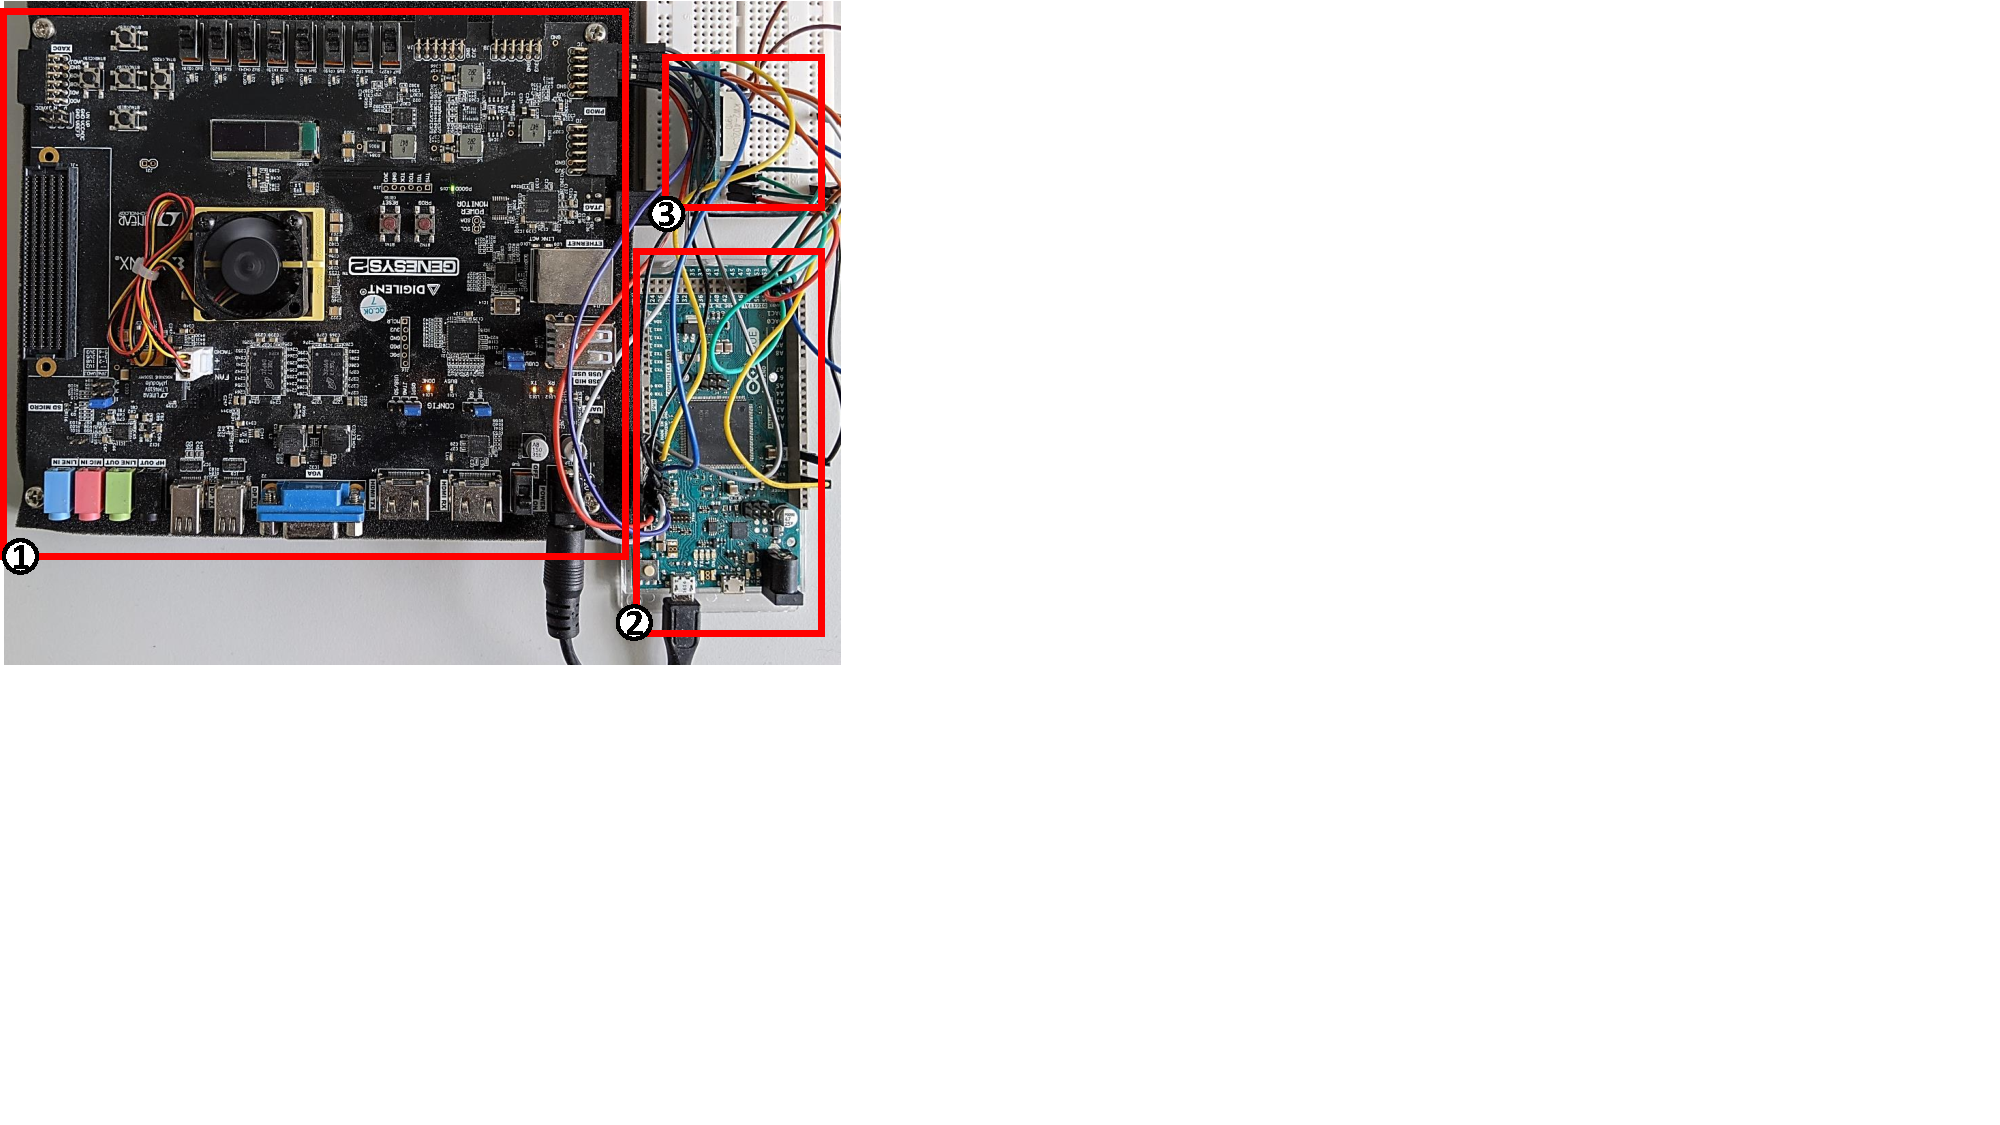
\includegraphics[trim={0 8cm 19cm 0}, clip, width=\linewidth]{chapters/PIE/images/prototype.pdf}
\caption[\name prototype]{The figure shows different components of our prototype: \one Digilent Genesys 2 FPGA board, \two Arduino Due as the peripheral simulator, and \three a seven-segment display unit as an example peripheral.} 
\label{fig:prototype}
\end{figure}

\subsection{Implementation}
\subsubsection{FPGA prototype}
\label{sec:eval:prototype}
We implemented an end-to-end prototype of \name that is based on the Keystone enclave framework~\cite{keystone}. Figure~\ref{fig:prototype} shows a case study on a platform that consists of an FPGA emulating the central processor connected to several Arduino boards that emulate \sphw. %We also discuss the added complexity in the form of trusted computing base of our prototype. Since added complexity is hard to quantify, we fall back on the metric ``lines of code'' for the TCB. 

\paragraph{FPGA platform}
We base our system on the Ariane core~\cite{ariane}, an open-source RISC-V 64-bit core that supports commodity OS such as Linux. It is an RC64GC 6-stage application class core that has been taped out multiple times and can operate up to 1.5 GHz. We run this core on a Digilent Genesys 2 FPGA board (\one in~\Cref{fig:prototype}).

We added PMP capability to the core that originally does not support PMP using 160 lines of SystemVerilog. The PMP unit is formally verified against a handwritten specification with yosys~\cite{wolf2016yosys}. Two of these units are inserted into the memory management unit (MMU) and are responsible for checking data accesses and instruction fetches. An additional unit is placed in the hardware page table walker to check page table accesses.
Our implementation has a configurable number of PMP entries up to the maximum number of 16 mandated by the standard~\cite{riscv2019privspec}. Our modifications have been contributed to the Ariane project and are open source~\cite{arianegithub}. Note that PMP is part of the RISC-V privilege standard and as such is already available on many other cores~\cite{asanovic2016rocket,ibex}. 

\paragraph{Processor-local enclaves}
%\name prototype leverages Keystone enclave framework~\cite{keystone} that uses a low-level trusted security monitor to run enclaves. 
We modified the SM to be able to connect two enclaves or an enclave and \sphw. Specifically, we added three new interfaces to the SM called \texttt{connect}, \texttt{sync\_disconnect}, and \texttt{async\_disconnect}. These interfaces can be used to set up shared regions between two enclaves or \sphw specified by their identifier. We also modified Keystone's attestation procedure to include a list of identifiers for all connected enclaves. Our modifications only amount to 390 additional or modified lines of code. The SM consists of around 2000 lines of code excluding SHA3 and ed25519 implementations that contribute around 4000 additional lines of code. %Our extension thus amounts to 9\% of added lines of code to Keystone (and 4.5\% including the crypto libraries).

In Keystone, every enclave runs on top of a minimal runtime that handles syscalls and manages virtual memory. Hence, its code is critical and part of the TCB. For our prototype, we added support to dynamically map shared memory regions into the virtual address space of an enclave. We modified 213 LoC out of a total of 3600 LoC for Keystone's runtime.

On the untrusted OS side, there are many components to make it easier to create and run enclaves such as an SDK and a kernel driver. These components also required numerous changes. However, they are not trusted and as such do not increase the TCB. 

\paragraph{Simple \sphw}  In our prototype, we emulated the a number of simple \sphw (e.g., keyboard, mice, simple sensors, etc.) on the Arduino Due microcontroller prototyping board (\two in Figure~\ref{fig:prototype}) using Arduino HID library. The Due's GPIO pins are connected to the FPGA's PMOD pins over two pairs of $8$ wires for bi-directioanl data. We modify the $I^2C$ protocol to communicate data between the Due and the FPGA. The physical limitations of the PMOD pins restricts the channel's frequency to $8$ MHz yielding 1 MB/s bandwidth. In the real world, the physical interfaces between the \sphw and the platform could be diverse such as USB, PCI-E, etc. As a concrete example, we implemented a keyboard with the Arduino board and wrote a simple keyboard driver that interprets the GPIO signal from the Arduino. Additionally, we use a PMOD interface-based seven-segment display unit as an output peripheral (\three in Figure~\ref{fig:prototype}). The driver contains around 50 LoC and is incorporated into our example controller enclave. Additionally, we use the \texttt{USBHost} library that can emulate a number of USB peripheral devices on the Arduino. We use the Arduino cryptographic library for signing the challenge messages from the \ce during the local attestation. The Due uses 128-bit AES (CTR mode) for encryption, HMAC\_SHA256 for message authentication, Curve25519 for key exchange, and SHA3 for the hash function. We use \texttt{DueFlashStorage} library to implement the NVM flash that contains the key materials for the peripheral attestation. Our prototype implementation is approximately 2.5K lines of code.

\subsubsection{Accelerator}
\label{sec:eval:accel}

We conduct another case study to show how complex \sphw such as a GPU-scale accelerator~\cite{zaruba2020manticore} can be extended to support \name. The accelerator is a 4096-core RISC-V platform that has comparable performance to current state-of-the-art machine learning accelerators. It is organized in clusters each with 8 individual single-stage RISC-V cores~\cite{zaruba2020snitch}, each of which is accompanied by a double precision floating point unit capable of two double precision and four single precision flops per cycle. To hide memory latency, all clusters have access to a scratchpad memory and a large L2 data cache. 

To provide multi-tenant isolation on the accelerator, we introduce a shared PMP unit with 4 entries into every cluster. The PMP entries can only be configured by one out of eight cores but the access policies will be enforced on all of them. With this additional hardware support we were able to implement a small firmware that configures the PMP entries according to the specifications from the host and then runs a task in user mode. Upon a context switch, the scratchpad memory that was in use by the previous task must be flushed and the PMP entries must be reconfigured. The firmware consists of 143 lines of assembly and 73 lines of C code. This implementation and verification takes around 3 weeks.

\subsection{Performance}
\label{sec:eval:numbers}
We list \name{}'s performance in the following categories:




% In traditional TEEs, the enclaves communicate through the untrusted operating system. Therefore, they first have to perform local attestation to establish a shared key which is then used to encrypt every message. Contrary to traditional TEEs, in \name, the enclaves establish a shared memory region to communicate directly. Hence, they do not need to encrypt messages as only the communicating enclaves have access to that shared memory. The shared memory enables the communication between enclaves to achieve the same performance what the memory bus could provide. 
% %This also requires some work by the SM similar to the local attestation for traditional enclaves. Thus, one approach requires encryption and the other does not. Since our platform does not support any kind of hardware acceleration for encryption algorithms, the performance difference between the two approaches would be huge. Therefore, we do not believe a comparison between these two systems is meaningful. 
% Recent work also shows the performance gains that can be extracted from enclave to enclave communication using shared memory~\cite{yu2020elasticlave}.

\begin{figure}[t]
    \centering
    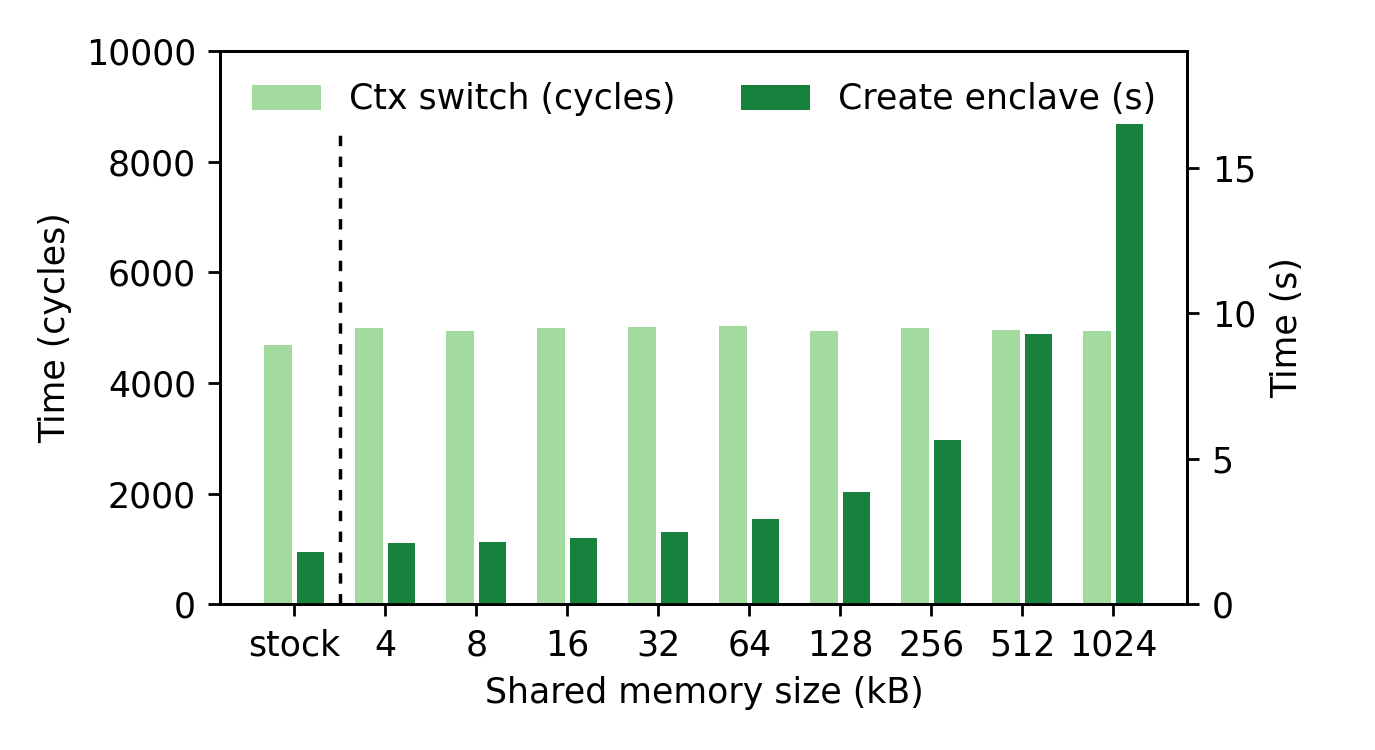
\includegraphics[width=\linewidth]{chapters/PIE/images/graphs/ctxswitch.png}
    \caption[Context switch performance]{Context switch performance for varying sizes of a shared memory region compared to stock Keystone performance on the left (equivalent to no shared memory).}
    \label{fig:ctxswitches}
\end{figure}


\begin{enumerate}
\item \textbf{Performance of enclave communication}
%A comparison between traditional enclave communication and our shared memory model is quite pointless. 
Since \name{} supports shared memory to communicate, its communication speed is the same as what the memory bus provides. This is much faster compared to traditional TEEs, where enclaves communicate through the OS requiring extra encryption steps. Concurrent work also demonstrates the performance gains that can be extracted from enclave to enclave communication using shared memory~\cite{yu2020elasticlave}.


\item \textbf{Context switches}
Context switches are critical for any system and determine its responsiveness and a part of its performance.
We performed experiments for various sizes of shared memory region and gathered various context switch latencies in \Cref{fig:ctxswitches}. We also measured the time of enclave creation which is mostly dominated by copying all the enclave data from the untrusted OS to the protected memory region and thus is expected to be linear in terms of shared memory size. 

These measurements highlight that the context switches are independent on the shared memory size. The absolute context switch time increases from 4730 for stock Keystone to 4950 for \name{}.
% We report that the performance within an enclave in our prototype is equivalent to the performance of stock Keystone~\cite{keystone}. This is reasonable since we do not modify anything that would affect Keystones performance.

\begin{table}[tbp]
    \centering
    \caption[Hardware size over of \name over the Ariane core]{\textbf{Hardware size over of \name over the Ariane core}Size of the default configuration of the Ariane core in gate equivalents (GE), synthesized in 22nm at 1GHz with varying number of PMP entries.}
    \begin{tabular}{llll}\toprule
        PMP entries & logic & caches & total \\\midrule
        0 & 472k GE & 686k GE & 1141k GE \\
        8 & 497k GE & 686k GE & 1164k GE \\
        16 & 531k GE & 686k GE & 1197k GE \\ \bottomrule
        % Overhead & 12.4\% & 0\% & 4.9\% \\ \bottomrule
    \end{tabular}
    
    \label{tab:eval:ariane}
\end{table}


\item \textbf{PMP overhead}
We measure the hardware overhead of PMP units in terms of the logic, the caches, and the total amount in NAND2 gate equivalents within the processor pipeline for 0, 8, and 16 PMP entries, and present them in \Cref{tab:eval:ariane}. We instantiate the Ariane core~\cite{ariane} with the default configuration: including the floating point unit, 32KiB L1 data cache, 16KiB L1 instruction cache, branch history table of size 64, and a 16-entry branch target buffer. We synthesized this instantiation of the core in a 22nm technology at 1GHz. %In order to provide a meaningful comparison, we provide the separate size of the logic, the caches, and the total amount in NAND2 gate equivalents in \Cref{tab:eval:ariane}. 

\item \textbf{Simple \sphw} The communication overhead between the platform and the peripheral device emulated by the Arduino due is very small. At the time of initialization, the peripheral and the platform exchanges handshake messages to perform local attestation. The initial handshake message is $60$ bytes. Every message size of our modified $I^2C$ protocol is 32 bytes. The combined latency introduced by signing averages around 60 $\mu$s.

\item \textbf{Accelerator} Our modification of the accelerator cores increases size by around 15\% and slows down from 750MHz to 666MHz due to the impact of the PMP access checks on the critical path. Note that this may not reflect the general case but rather reflects an upperbound. The change in area of a single core complex (core, FPU, and an integer subsystem) can be found in \Cref{tab:areasnitch}. In total, the area of the entire accelerator only increased by around 0.6\%, with most of the area being occupied by the floating point units.
%The implementation and verification of the firmware took another engineering week. 
\end{enumerate}



\begin{table}[tbp]
\centering
\caption[The area rundown of our modifications to the accelerator]{\textbf{The area rundown of our modifications to the accelerator.} The area rundown of our modifications to the accelerator with 4 and 0 PMP entries respectively. Synthesized in 22nm with 750MHz clock for 0 entries and 666MHz with 4 entries. Area given in $\mu m^2$.}
\label{tab:areasnitch}
\begin{tabular}{@{}lccc@{}}
\toprule
\multirow{2}{*}{Area {[}$\mu$m$^2${]}} & \multicolumn{2}{c}{\#PMP entries} & \multirow{2}{*}{Overhead} \\ & 0                 & 4                 &\\ \midrule
Core   & 5.7               & 6.7               & 15.5\%                    \\
FPU    & 39.2              & 37.9              & -3.3\%                    \\
IPU   & 8.6               & 8.5               & -1.4\%                    \\ \midrule
Total  & 53.5              & 53.2              & -0.7\%                    \\ \bottomrule
\end{tabular}
\end{table}

% 
% \begin{figure}
%     \centering
%     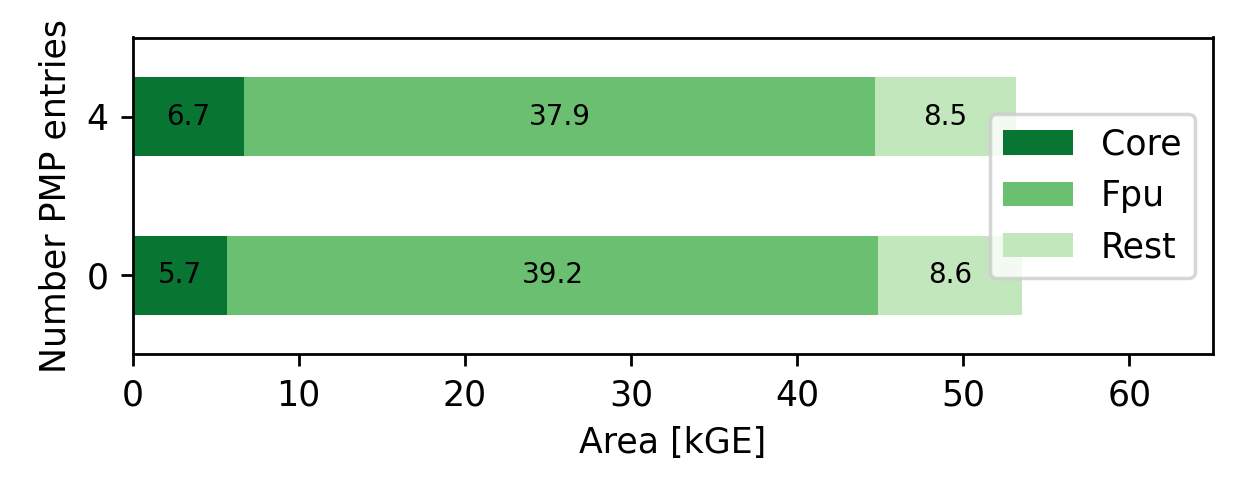
\includegraphics[width=0.9\linewidth]{chapters/PIE/images/graphs/areasnitch.png}
%     \vspace{-1em}
%     \caption[The post-synthesis area of a core complex of our accelerators]{The post-synthesis area of a core complex of our accelerators, with four and zero PMP entries respectively. Note that the design was synthesized with 750MHz clock for 0 PMP entries and 666MHz with 4 entries. The size of the core increases due to the increased pressure by the PMPs, while the FPU gets smaller with the lower clock as its critical path is not affected by the PMP entries.}
%     \label{fig:areasnitch}
% \end{figure}

\setcounter{para}{0}



